% KWEB Del 1.1 (WP1.1) Report
%

\documentclass[a4paper,twoside,12pt]{report}
\usepackage{times}
\usepackage{graphics}
%\usepackage{graphicx}
%\usepackage{epsfig}
%\usepackage[]{graphicx}
\usepackage{deliverable}
%\usepackage{pnamed}

%cabeceras

\usepackage[T1]{fontenc}
% españolización
\usepackage[english]{babel}
\usepackage[utf8]{inputenc}
\usepackage{rotating}
\usepackage{graphicx}
\usepackage{color}
\usepackage{xspace}
% mejoras visuales
\usepackage{enumerate}
\usepackage{fancyhdr}  % para configurar los encabezados
\usepackage{fancybox}  % para hacer cajitas
\usepackage[normal,oneline,sf,bf]{caption2}
\usepackage{titlesec}  % para configurar los títulos de sección
\usepackage{paralist}
\usepackage{url}
\usepackage{latexsym}
\usepackage{amsmath}
\usepackage{amssymb}
\usepackage{amsthm}

\usepackage{epigraph}

% citas, referencias e índices
\usepackage{cite}
%\usepackage{citesort}   % da errores al compilar
\usepackage{makeidx}

% incrustaciones de código fuente
%\usepackage[norules,nolineno]{lgrind}
\usepackage{verbatim}
\usepackage{listings}
%\usepackage{noweb,a4wide}


%\usepackage{textcomp}
\usepackage[right]{eurosym}

% columnas
\usepackage{multicol}

% tablas
\usepackage{longtable}

%\input{commands}

% \addto\captionsspanish{
%         \def\listtablename{\'Indice de tablas}%
%         \def\tablename{Tabla}} 



\lstset{%
        language=Java,
	basicstyle=\footnotesize\sffamily,
	keywordstyle=\bfseries, %\color{darkred}
 	stringstyle=\itshape, %\color{violet}
 	commentstyle=\itshape, %\color{blue}
 	showspaces=false,
 	showtabs=false,
 	showstringspaces=false,
 	frame=trBL,
        frameround=tttt,
        %backgroundcolor=\color{lightyellow},
 	extendedchars=true,
 	numbers=none,
        aboveskip=0.5cm,
        belowskip=0.5cm,
        xleftmargin=1cm,
        xrightmargin=1cm,
	breaklines=true,
        morekeywords={PREFIX,java,rdf,rdfs,url,dcterms,foaf,skos,gr,skosxl}
}
\definecolor{darkred}{rgb}{0.5, 0, 0}
\definecolor{violet}{rgb}{1, 0, 1}
\definecolor{lightyellow}{rgb}{1,1,0.8}


\newtheorem{theorem}{Theorem}[section]
\newtheorem{proposition}[theorem]{Proposición}
\newtheorem{lemma}[theorem]{Lema}
\newtheorem{definition}[theorem]{Definición}
\newtheorem{examples}[theorem]{Ejemplo}
\newtheorem{remarks}[theorem]{Remarks}
\newtheorem{corollary}[theorem]{Corolario}
\newtheorem{remark}[theorem]{Remark}
\newtheorem{example}[theorem]{Ejemplo}
\newtheorem{conjecture}[theorem]{Conjecture}
\newtheorem{note}[theorem]{Nota}



\begin{document}

\title{Quality Management in Service-based Systems and Cloud Applications}

\author{
{Jose María Alvarez-SEERC\\
jmalvarez@seerc.org \\
josem.alvarez@josemalvarez.es}}

\revised{September 30, 2013}

%\issuer{Vrije Universiteit Amsterdam}

\identifier{WP4-SEERC-ER-TR}

\version{v1.0}

\state{Final}

\project{WP4‐Quality Management and Business Model Innovation}

\distribution{protected}

\synopsis{\strut\\
The FP7 Marie Curie Initial Training Network ``RELATE''  \\
Technical Report.

Keywords: cloud computing, services quality, semantics
}

\coverpages

\setcounter{page}{0}

\pagenumbering{roman}

\include{historial}
\include{resumen}

\setlength{\parskip}{0.0cm}
\tableofcontents
\listoffigures
\listoftables
\setlength{\parskip}{1.0ex}

\newpage
\pagenumbering{arabic}


%%%%%%%%%%%%%%%%%%%%%%%%%%%%%%
%\pagestyle{kweb}

%\chapter{Introduction}
Cloud Computing~\cite{mell2011nist} systems and Service Oriented Architectures (SOA) have 
reached a level of complexity~\cite{Huebscher:2008:SAC:1380584.1380585,Conejero:2012:MSQ:2357487.2357591} that implies the necessity of new methods 
and algorithms to automatically deal with the vast amount of data, variables, 
parameters, etc. that appears in this new realm for the advanced management of 
applications, services or resources. 

In this new environment QoS is playing a relatively minor role but its 
importance, in a wide range of applications scenarios, is likely become more 
crucial than ever before. In recent years and due to the deployment of web 
services a considerable research effort in QoS has been made. However existing 
QoS mechanisms are actually available in a few large scale commercial 
environments and with a limited extent. The main problem lies in the complexity 
of designing QoS models that enables an adequate management of a distributed 
architecture making decisions about resource provisioning, getting feedback for 
the final users, etc. with the objective of avoiding existing ``brute-force''
solutions and overprovisioning. 

Although QoS management has been also widely investigated~\cite{Conejero:2012:MSQ:2357487.2357591} 
in the well-known grid-computing area the emergence of the Cloud Computing paradigm 
brings a new set of open issues: accomplish the  Service Level Agreements (SLAs), predict 
future workload, process large and diverse data streams/logs, make real-time 
decisions, reasoning and inference, dynamic adaptation and provision of 
resources, etc. In the widely-accepted definition~\cite{mell2011nist} of 
he National Institute of Standards and Technology (NIST) QoS 
would be aligned to the concept of ``Measured Service'', see Figure~\ref{fig:qos-intro}, and more specifically to define both characteristics applicable to a service and operations 
to be delivered such as predictive analysis. The aforementioned points are very challenging and should be 
addressed in order to ease an intelligent, flexible and self-managing system of cloud-based applications and platforms.

% 
 \begin{figure}[!ht]
\centering
	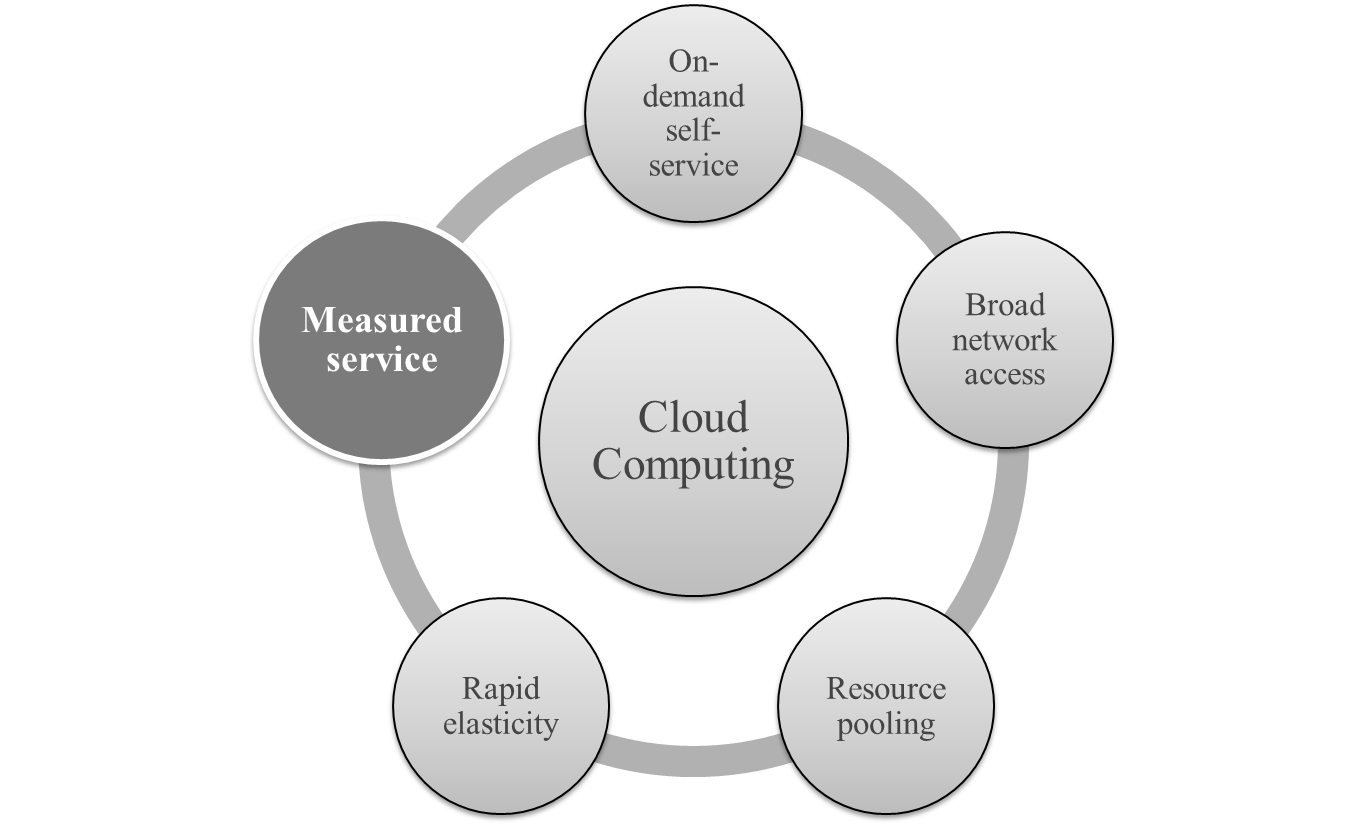
\includegraphics[width=12cm]{./imgs/qos-intro}
 \caption{Quality of Service in the NIST definition~\cite{mell2011nist}.}
 \label{fig:qos-intro}
\end{figure}

Furthermore a proper management of a cloud system taking into account QoS 
features can save costs, keep high-performance, reserve resources on-demand and 
offer a user-friendly experience to both IT managers and final users. 
Traditionally, QoS has been handled using a combination of network resource 
provisioning with techniques such as admission control or active queue 
management. Nowadays these old-fashioned techniques can be applied to a static 
environment but in the near future with the new implications for professionals~\cite{DBLP:journals/jucs/Colomo-PalaciosFSS12}, 
the challenge of providing higher elasticity and dynamic adaptation cannot be accomplished with these methods. In this sense it is clear that QoS will remain a fundamental requirement in the next wave of 
applications and services on the Web and there is no doubt that QoS should 
address the new challenges applying emerging and trending technology and 
approaches to overcome existing restrictions in QoS models.

The features and requirements of these new cloud systems with regards 
to QoS~\cite{Pedersen:2011:AMQ:2114495.2115542} and their implications in the future IT~\cite{DBLP:journals/jucs/Colomo-PalaciosFSS12} 
match the advantages of software component and knowledge-based architectures. In fact, Autonomic Computing support for the next generation of cloud systems 
needs to be~\cite{Conejero:2012:MSQ:2357487.2357591,Pedersen:2011:AMQ:2114495.2115542}: 
1) Self-x management, 2) agile, flexible and reliable, 4) deployable over a multiple cloud platforms, 5) handle complexity, 6) enable 
collaboration and coordination and 7) cost-effective and greener 
(energy-efficient). Under this context, semantic technologies have emerged as an 
option to design and develop intelligent software components and agents to 
perform certain tasks on the Web and fulfill user's requirements (in this case 
applications). Therefore, Semantics enables machines to automatically process 
and enrich data from different sources and has the potential to deeply influence 
the further development of the Internet Economy as cloud systems also does.

In the Semantic Web area, there is a growing commitment to process large data streams applying 
new stream reasoning~\cite{Bolles:2008:SSE:1789394.1789438,Barbieri:2010:EEC:1739041.1739095} 
or complex event processing~\cite{Anicic:2011:EUL:1963405.1963495} (CEP) techniques. Furthermore there are research works offering cloud-based 
solutions to deal with Big Data~\cite{Fan:2013:MBD:2481244.2481246} (e.g. analysis of social media), modeling SLAs and ECA rules with ontologies, 
monitoring real-time systems (e.g. traffic), sensor networks, or making decisions in a collaborative fashion~\cite{RodriGuez-GonzaLez:2012:UAP:2350799.2350907} (e.g. clinical reasoning). 
The main advantage of applying semantic technologies to a specific domain lies in the standard representation of knowledge and data through a common-shared data model (RDF) and the 
capacity of reusing existing knowledge through ontologies (OWL). Thus, data coming from cloud systems can be automatically processed, checked for inconsistencies and 
used in expert systems to support self-x management activities.

This review is intended to provide researchers, developers and practitioners a summary of the current status of QoS management in Cloud Computing and SOA applying semantics. To do so, the paper 
is structured as follows. Next section reviews the background concepts required to a better understanding of the paper. Section~\ref{qos-semantics} 
presents the existing works to perform QoS management using semantics; more specifically most of the ontology-based frameworks for 
QoS management are reviewed. Afterwards, a review of existing techniques for processing large data streams is also provided in Section~\ref{data-stream}. 
Section~\ref{framework} outlines a framework to meet QoS requirements applying semantics and data stream processing techniques in real-time. 
Finally, the paper ends with a discussion of existing approaches for semantic-based QoS management, 
limitations, future challenges and concluding remarks. 


%\input{chapters/consideraciones-generales}
% \input{chapters/personas}
%\input{localidades}
%\input{documentos}
%\input{organizaciones}
%\input{roles}
%\input{eventos}
%\input{proyectos-ley}

\bibliographystyle{unsrt}
% \bibliography{AEN01-00}

\end{document}
